%%%
% Denne fil indeholder noter til Kontekstfrie Sprog (Kapitel 2 i Sipser)
% Derudover indeholder den også mine løsninger til opgaver om kontekstfrie sprog.
% Opgaver:
% TODO: Kapitel 2.2
% TODO: Kapitel 2.3
%%%
\chapter{Kontekstfrie Sprog}

I det tidligere kapitel om endelige automater, så vi den klasse af sprog som de genkender, regulære sprog, men vi så også eksempler på sprog som ikke er regulære, og hvordan dette kan bevises. I dette kapitel vil vi introducere \textit{kontekstfrie grammatikker} som er stærkere end endelige automater i deres deskriptionskraft. Sprogene der genkendes af kontekstfrie grammatikker kaldes \textit{kontekstfrie sprog}. Ydermere introducerer vi \textit{stakautomater} (pushdown automata på engelsk) som er en klasse af maskiner der genkender kontekstfrie sprog.

\section{Kontekstfrie Grammatikker}
En grammatik består af en samling af \textbf{substitueringsregler}, også kaldet \textit{produktioenr}. Hver regel forekommer som en linje i grammatikken,  og består af et symbol efterfulgt af en pil efterfulgt af en streng. Følgende grammatik er et eksempel på en kontekstfri grammatik $G_{1}$:
\begin{equation}
  \tag{$G_{1}$}
  \begin{split}
  A &\rightarrow \mathtt{0}A \mathtt{1}\\
  A &\rightarrow B\\
  B &\rightarrow \mathtt{\#}
\end{split}
  \label{eqn:G1}
\end{equation}

Symbolet på venstresiden kaldes en \textit{variabel}\footnote{Kært barn har mange navne, jeg har også hørt non-terminal og, simpelt, LHS.}. Strengen (højresiden) består af variabler og andre symboler, kaldet \textit{terminale}. Terminale minder om alfabetet fra en endelig automat, da disse er de endelige symboler, der udgør en resulterende streng\footnote{Dette vil vi komme ind på i mere detalje senere.}. Variabler er oftest repræsenteret som store bogstaver, hvor terminale kan være små bogstaver, tal, eller specielle symboler (såsom \#.) En af variablerne (venstrehåndssiden) bliver udpeget til at være \textbf{startvariablen}. Denne variabel skal alle udledninger\footnote{En udledning bliver beskrevet i mere detalje i næste afsnit.} af grammatikken starte på (analogt til en start state i en endelig automat.)

For at beskrive et sprog med en grammatik, \textit{udleder} vi strenge fra grammatikken. Dette bliver gjort systematisk ved at \textit{substituere} variabler med andre variabler eller terminale. Eksempeltvis kan gramatikken \ref{eqn:G1} udlede strengen \texttt{000\#111}. En udledning af denne streng i \ref{eqn:G1} er følgende: $A \Rightarrow \mathtt{0}A \mathtt{1} \Rightarrow \mathtt{00}A \mathtt{11} \Rightarrow \mathtt{000}A \mathtt{111} \Rightarrow \mathtt{000}B \mathtt{111} \Rightarrow \mathtt{000\#111}$. En måde hvorpå du kan vise dette grafisk er \textit{parse-træer}. Et eksempel kan ses i Figur~\ref{fig:parsetreeg1}, som viser et parsetræ for strengen \texttt{000\#111} i grammatikken \ref{eqn:G1}.

\begin{figure}[ht]
  \centering
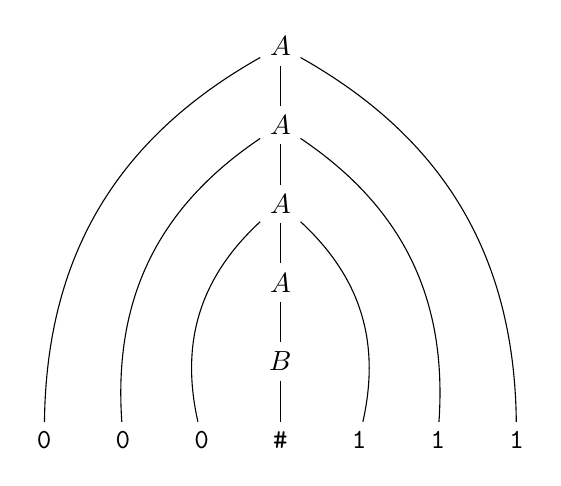
\begin{tikzpicture}[>=latex]
  % Nodes
  \node (0a) at (0,0) {\texttt{0}};
  \node (0b) at (1,0) {\texttt{0}};
  \node (0c) at (2,0) {\texttt{0}};
  \node (sharp) at (3,0) {\texttt{\#}};
  \node (1a) at (4,0) {\texttt{1}};
  \node (1b) at (5,0) {\texttt{1}};
  \node (1c) at (6,0) {\texttt{1}};

  % Upper nodes
  \node (B) at (3,1) {$B$};
  \node (A4) at (3,2) {$A$};
  \node (A3) at (3,3) {$A$};
  \node (A2) at (3,4) {$A$};
  \node (A1) at (3,5) {$A$};

  % Lines going down
  \draw[-] (B) to (sharp);
  \draw[-] (A4) to (B);
  \draw[-] (A3) to (A4);
  \draw[-] (A2) to (A3);
  \draw[-] (A1) to (A2);

  % Lines going to terminals
  \draw[-] (A1) to[bend right] (0a);
  \draw[-] (A1) to[bend left] (1c);
  \draw[-] (A2) to[bend right] (0b);
  \draw[-] (A2) to[bend left] (1b);
  \draw[-] (A3) to[bend right] (0c);
  \draw[-] (A3) to[bend left] (1a);

\end{tikzpicture}
  \caption{\label{fig:parsetreeg1} Parse-træ for \texttt{000\#111} i \ref{eqn:G1}}
\end{figure}


Alle strenge du kan udlede på denne måde er en del af sproget, og udgør tilsammen det kontekstfri sprog som \ref{eqn:G1} genkender. Hvis du ikke har lagt mærke til det nu, er denne meget simple kontekstfri grammatik faktisk et eksempel på et sprog der \textbf{ikke} kan genkendes af en endelig automat. Ofte, fremfor at skrive $A \rightarrow \mathtt{0}A \mathtt{1}$ og så på en ny linje skrive $A \rightarrow B$, så skriver man blot $A \rightarrow \mathtt{0} A \mathtt{1} | B$, hvor du kan se \texttt{|} som ``eller''.

Vi vil nu kigge på den formelle definition på en kontekstfri grammatik.

\begin{definition}[Formel Definition på en Kontekstfri Grammatik]
  En \textbf{kontekstfri grammatik}   er en 4-tuple $(V, \Sigma, R, S)$, hvor
  \begin{enumerate}
    \item $V$ er et endeligt sæt kaldet \textbf{variabler}
    \item $\Sigma$ er et endeligt sæt, disjunkt fra $V$, kaldet \textbf{terminaler}
    \item $R$ er et endeligt sæt af \textbf{regler}, hvor hver regel er en streng af variabler og terminaler og en variabel
    \item $S \in V$ er startvariablen.
  \end{enumerate}

\end{definition}

Givet $u, v$ og $w$ er strenge af variabler, og terminale, og $A \rightarrow w$ er en regel af grammatikken, så siger vi at $uAv$ giver (\textit{yields}) $uwv$, skrevet $uAv \Rightarrow uwv$. Vi siger at $u$ udleder $v$, skrevet, $u \stackrel{*}{\Rightarrow} v$, hvis $u = v$, eller hvis en sekvens $u_{1}, u_{2}, \ldots, u_{k}$ eksisterer når $k \geq 0$ og $u \Rightarrow u_{1} \Rightarrow u_{2} \Rightarrow \ldots \Rightarrow u_{k} \Rightarrow v$. Sproget af grammatikken er $\{w \in \Sigma* | S \stackrel{*}{\Rightarrow} w\}$.

Altså betyder det, at hvis $u$ \textit{giver} $v$, så tager det kun ét skridt. Hvis $u$ \textit{udleder} $v$ tager det mere end ét skridt.

\newpage
\subsection{Tvetydighed}%
\label{sub:tvetydighed}

En grammatik der kan generere den sammen streng på to eller flere forskellige måder (og dermed have mere end ét parsetræ for én streng), kaldes \textit{tvetydig}. For eksempel er den følgende grammatik tvetydig:
\[
\langle EXPR \rangle \rightarrow \langle EXPR \rangle + \langle EXPR \rangle | \langle EXPR \rangle + \langle EXPR \rangle | ( \langle EXPR \rangle ) | a
\]

Strengen $\mathtt{a + a \times a}$ kan genereres tvetydigt, enten: $$\langle EXPR \rangle \Rightarrow \langle EXPR \rangle + \langle EXPR \rangle \Rightarrow \langle EXPR \rangle + \langle EXPR \rangle \times \langle EXPR \rangle \Rightarrow \cdots \Rightarrow a + a \times a$$ eller $$\langle EXPR \rangle \Rightarrow \langle EXPR \rangle \times \langle EXPR \rangle \Rightarrow \langle EXPR \rangle + \langle EXPR \rangle \times \langle EXPR \rangle \Rightarrow \cdots \Rightarrow a + a \times a$$.

\begin{definition}[Tvetydighed]
En streng $w$ er udledt \textbf{\textit{tvetydigt}} i en kontekstfri grammatik $G$ hvis den har to eller flere venstremest udledninger. Grammatik $G$ er \textit{tvetydig} hvis den genererer en streng tvetydigt.
\end{definition}

Ofte, hvis man har en tvetydig grammatik, er det muligt at konvertere den til en grammatik der ikke er tvetydig. Dog er dette ikke muligt for alle sprog. Sprog hvor dette \textbf{ikke} gælder kalder vi \textbf{i sig selv tvetydige} (inherently ambiguous.)

\newpage
\subsection{Chomsky Normal Form}%
\label{sub:cnf}

Chomsky Normal Form er en simple form af en kontekstfri grammatik.

\begin{definition}[Chomsky Normal Form]
  En kontekstfri grammatik er i \textbf{\textit{Chomsky Normal Form}} hvis hver regel har formen
  \begin{equation*}
\begin{split}
  A &\rightarrow BC\\
  A &\rightarrow a
\end{split}
  \end{equation*}
  hvor $a$ er enhver terminal, og $A, B$ og $C$ er enhver variabel, dog må $B$ og $C$ ikke være startvariablen. Derudover tillader vi reglen $S \rightarrow \varepsilon$, hvor $S$ er startvariablen.
\end{definition}

\begin{theorem}
Ethvert kontekstfri sprog er genereret af en kontekstfri grammatik i Chomsky Normal Form.
\end{theorem}

Vi vil vise at vi kan konvertere enhver grammatik til chomsky normal form. Vi vil gøre dette ved at fjerne alle regler der går imod betingelserne for CNF, og erstatte med regler der overholder. Først tilføjer vi en ny startvariabel, og eliminerer alle regler af formen $A \rightarrow \varepsilon$ (kaldet $\varepsilon$-regler.) Vi eliminerer også alle \textbf{unit rules}, som har formen $A \rightarrow B$. Til sidst konverterer vi resten til at være i ordentlig form.

\begin{proof}
  \noindent
  \textbf{\large Skridt 1:} Først tilføjer vi en ny variabel $S_{0}$ og reglen $S_{0} \rightarrow S$, hvor $S$ er det originale startvariabel.

  \noindent
  \textbf{\large Skridt 2:} Efter dette fjerner vi alle regler af formen $A \rightarrow \varepsilon$, hvor $A \neq S$. Når dette er gjort fjerne vi alle regler hvor $A$ er på højresiden af en regel, og tilføjer en ny regel med $A$ fjernet. Eksempelvis bliver $R \rightarrow uAv$ til $R \rightarrow uv$ og $R \rightarrow uAvAw$ bliver til tre regler $R \rightarrow uvAw, R \rightarrow uAvw, R \rightarrow uvw$. Hvis vi har reglen $R \rightarrow \varepsilon$ tilføjer vi $R \rightarrow \varepsilon$, \textbf{undtagen hvis vi allerede har fjernet denne regel.} Vi forstætter dette indtil alle $\varepsilon$-regler er væk (undtagen startvariablen.)

  \noindent
  \textbf{\large Skridt 3:} Efter vi har gjort dette tager vi os af \textit{unit rules}. Vi fjerner en unit rule $A \rightarrow B$. Så, når $B \rightarrow u$ forekommer, tilføjer vi $A \rightarrow u$ (bemærk at vi ikke fjerner $B \rightarrow u$, da den kan komme et andet sted fra.) Vi bliver ved indtil vi har fjernet alle unit rules.

  \noindent
  \textbf{\large Skridt 4:} Til sidst konverterer vi resten af reglerne til den rigtige form. Vi erstatter hver regel $A \rightarrow u_{1}u_{2} \cdots u_{k}$ hvor $k \geq 3$ og hvert $u_{i}$ er en variabel eller terminalt symbol, med reglerne $A \rightarrow u_{1}A_{1}, A_{1} \rightarrow u_{2}A_{2}, A_{2} \rightarrow u_{3}A_{3}, \ldots, $ og $A_{k-2} \rightarrow u_{k-1}u_{k}$.  $A_{i}$'erne er nye variabler. Vi erstatter en hver terminal $u_{i}$ i de tidligere regler men den nye variabel $U_{i}$ og tilføjer reglen $U_{i} \rightarrow u_{i}$.
\end{proof}

Dette kan godt være svært at forstå, og derfor kigger vi på et eksempel.

\begin{example}
  Vi konverterer følgende grammatik til CNF:

\begin{equation*}
\begin{split}
  S &\rightarrow ASA\;|\;aB \\
  A &\rightarrow B\;|\;S \\
B &\rightarrow b\;|\; \varepsilon
\end{split}
\end{equation*}

\noindent
\textbf{\large Skridt 1}:\\
\noindent
Første skridt er at tilføje en ny startvairabel. Vi gør dette ved at introducere reglen $S_{0} \rightarrow S$

\begin{equation*}
\begin{split}
  S_{0} &\rightarrow S\\
  S &\rightarrow ASA \;|\; aB\\
  A &\rightarrow B \;|\; S\\
  B &\rightarrow b \;|\; \varepsilon
\end{split}
\end{equation*}

\noindent
\textbf{\large Skridt 2:}\\
\noindent
Vi fjerner $\varepsilon-$reglerne.
\begin{equation*}
\begin{split}
  S_{0} &\rightarrow S\\
  S &\rightarrow ASA \;|\; aB \;|\; a\;\;\;\;\; \text{\color{gray}da B kan blive }\varepsilon\\
  A &\rightarrow B \;|\; S \; | \; \varepsilon\\
  B &\rightarrow b
\end{split}
\end{equation*}

\noindent
Dog introducerer dette en ny epsilon-regel som vi må fjerne:


\begin{equation*}
\begin{split}
  S_{0} &\rightarrow S\\
  S &\rightarrow ASA \;|\; aB \;|\; a \;| \;SA \;| \;AS \;| \;S\\
  A &\rightarrow B \;|\; S \\
  B &\rightarrow b
\end{split}
\end{equation*}

\noindent
\textbf{\large Skridt 3:}\\
\noindent
Vi fjerner nu unit-reglen $S \rightarrow S$:
\begin{equation*}
\begin{split}
  S_{0} &\rightarrow S\\
  S &\rightarrow ASA \;|\; aB \;|\; a \;| \;SA \;| \;AS \\
  A &\rightarrow B \;|\; S \\
  B &\rightarrow b
\end{split}
\end{equation*}
Og nu $S_{0} \rightarrow S$:


\begin{equation*}
\begin{split}
  S_{0} &\rightarrow ASA \;|\; aB \;|\; a \;| \;SA \;| \;AS \\
  A &\rightarrow B \;|\; S \\
  B &\rightarrow b
\end{split}
\end{equation*}

Nu fjerner vi reglen $A \rightarrow B$:
\begin{equation*}
\begin{split}
  S_{0} &\rightarrow ASA \;|\; aB \;|\; a \;| \;SA \;| \;AS \\
  A &\rightarrow  S  \;|\; b\\
  B &\rightarrow b
\end{split}
\end{equation*}

Til sidst fjerner vi reglen $A \rightarrow S$:
\begin{equation*}
\begin{split}
  S_{0} &\rightarrow ASA \;|\; aB \;|\; a \;| \;SA \;| \;AS \\
  A &\rightarrow  b  \;|\; ASA \;|\; aB \;|\; a \;|\; SA \;|\; AS \\
  B &\rightarrow b
\end{split}
\end{equation*}


\noindent
\textbf{\large Skridt 4:}\\
\noindent
Nu skal vi konvertere resten.

\begin{equation*}
\begin{split}
  S_{0} &\rightarrow AA_{1} \;|\; UB \;|\;a \;|\;SA \;|\; AS  \\
  S &\rightarrow AA_{1} \;|\; UB \;|\;a \;|\;SA \;|\; AS  \\
  A &\rightarrow  b  \;|\; AA_{1} \;|\; a \;|\; SA \;|\; AS \\
  A_{1} &\rightarrow SA \\
  U &\rightarrow a\\
  B &\rightarrow b
\end{split}
\end{equation*}

\end{example}

\section{Pushdown Automater}%
\label{sec:pushdownautomata}

Pushdown Automata (PDA) er ligesom NFA'er, men med en \textbf{stak} tilføjet. Denne stak tillader at PDA'en kan genkende kontekstfrie sprog. Det vil altså sige at en PDA er ækvivalent i dens kraft med kontekstfrie grammatikker.

\begin{figure}[ht]
  \centering
  \begin{tikzpicture}
    % Define the style for the blocks
    \tikzset{block/.style={rectangle, draw, minimum height=2em, minimum width=3em}}
    \tikzset{line/.style={draw, -latex'}}

    % Place the first block
    \node[block] (state) {state control};

    % Draw the input nodes
    \node[block, minimum width=0.8cm] (a1) at (2,-1.0) {a};
    \node[block, minimum width=0.8cm] (a2) at (2.8,-1.0) {a};
    \node[block, minimum width=0.8cm] (b1) at (3.6,-1.0) {b};
    \node[block, minimum width=0.8cm] (b2) at (4.4,-1.0) {b};


    \node[label] (input) at (5.5, -1.0) {input};

    \node[block, minimum width=0.8cm, minimum height=0.8cm] (x) at (1.5, -2.6) {x};
    \node[block, minimum width=0.8cm, minimum height=0.8cm] (y) at (1.5, -3.4) {y};
    \node[block, minimum width=0.8cm, minimum height=0.8cm] (z) at (1.5, -4.2) {z};

    \node[label] (stack) at (2.5, -3.4) {stak};

    \draw[->, thick] (state) -| (a1);
    \draw[->, thick] (state) |- (x);


  \end{tikzpicture}
  \caption{\label{fig:pda} Skematik af en pushdown automat}
\end{figure}

I Figur~\ref{fig:pda} ses en skematik af en PDA med en stak, hvor ``state control'' er delen med alle statesne, pile, etc. ``input'' er inputtet til automaten, og ``stak'' er stakken. En PDA kan skrive symboler til stakken og så læse dem tilbage senere. Den fungerer i en last-in-first-out princip. Vi referer i noterne til ``pushing'' som værende at give data til stakken, og ``popping'' som værende at læse data fra stakken.

\begin{example}
  Sproget $\{0^{n}1^{n} | n \ge 0\}$ kan \textbf{ikke} genkendes af en endelig automat, men det kan den af en PDA. Følgende er en beskrivelse af hvordan automaten fungerer:\\
  \noindent
  Læs symbolerne fra input. Hver gang et 0 bliver læst, pushes den til stakken. Hver gang et 1 er læst, pop den fra stakken. Hvis inputet er færdiglæst så snart stakken er tom, accepteres inputtet. Ellers accepteres det ikke (f.eks. hvis der er flere 1'ere når stakken er tom, hvis der er flere 0'ere efter der er fundet en 1'er, hvis stakken stadig har 0'ere.)
\end{example}

Det er vigtigt at bemærke at de pushdown automater vi arbejder med er nondeterministiske, da deterministiske og nondeterministiske pushdown automater \textbf{ikke} er ævkvivalente i deres kraft.

\subsection{Formel Definition af Pushdown Automat}%
\label{subsec:formelPDA}

Den formelle definition for en PDA minder meget om den for en FA, dog med et ekstra alfabet: $\Gamma$ som er alfabetet for stakken.

\begin{definition}[Formel Definition af en Pushdown Automat]
\label{def:pda}
En \textit{pushdown automat} er en 6-tuple $(Q, \Sigma, \Gamma, \delta, q_{0}, F)$, hvor $Q$, $\Sigma$, $\Gamma$, og $F$ alle er endelige sæt, og
\begin{enumerate}
  \item $Q$ er sættet af states
  \item $\Sigma$ er input alfabetet
  \item $\Gamma$ er stak alfabetet
  \item $\delta : Q \times \Sigma_{\varepsilon} \times \Gamma_{\varepsilon} \longrightarrow P(Q \times \Gamma_{\varepsilon})$ er transitionsfunktionen
  \item $q_{0} \in Q$ er start staten
  \item $F \subseteq Q$ er sættet af accept states.
\end{enumerate}

\subsection{Pushdown Automat Komputering}%
\label{subsec:PDAKomputering}


En PDA $M = (Q, \Sigma, \Gamma, \delta, q_{0}, F)$ komputerer som følger. Den accepterer input $w$ hvis $w$ kan skrives $w = w_{1} \cdots w_{m}$, hvor hvert $w_{i} \in \Sigma_{\varepsilon}$ og sekvensen af states $r_{0}, r_{1} \ldots, r_{m} \in Q$ og strenge $s_{0}, s_{1}, \ldots, s_{m} \in \Gamma^{*}$ eksisterer som tilfredsstiller følgene betinglser, hvor $s_{i}$ repreæsenterer sekvensen af stakindhold som $M$ har på den accepterende afdeling af komputering.
\begin{enumerate}
  \item $r_{0} = q_{0}$ og $s_{0} = \varepsilon$. Altså starter vi ved start staten og har en tom stak.
  \item For $i = 0, \ldots, m-1$ har vi $(r_{i+1}, b) \in \delta(r_{i}, w_{i+1}, a)$, hvor $s_{i} = at$ og $s_{i+1} = bt$ for alle $a, b \in \Gamma_{\varepsilon}$ og $t \in \Gamma^{*}$. Altså $M$ bevæger sig ifølge staten, stakken og inputsymbolet.
  \item $r_{m} \in F$. Den sidste state er en accept state.
\end{enumerate}

\subsection{Eksempler}%
\label{subsec:pdaeksempler}

\begin{example}[$\{0^{n}1^{n} | n \ge 0\}$]
  Vi kigger på et eksempel af en formel definition af en PDA der genkender sproget $\{0^{n}1^{n} | n \geq 0\}$.
  Lad $M_{1}$ være $(Q, \Sigma, \Gamma, \delta, q_{1}, F)$, hvor
  \begin{enumerate}
    \item $Q = \{q_{1}, q_{2}, q_{3}, q_{4}\}$.
    \item $\Sigma = \{0,1\}$
    \item $\Gamma = \{0, \$\}$
    \item $F = \{q_{1}, q_{4}\}$
    \item $\delta$ gives af følgende tabel, hvor tomme felter er $\emptyset$:
          \begin{center}
            % Please add the following required packages to your document preamble:
% \usepackage{multirow}
\begin{table}[ht]
\begin{tabular}{l|lllllllll}
\multirow{2}{*}{\begin{tabular}[c]{@{}l@{}}Input \\ Stak:\end{tabular}} & \multicolumn{3}{l|}{0}                                                                & \multicolumn{3}{l|}{1}                                                                  & \multicolumn{3}{l|}{$\varepsilon$}                                                     \\ \cline{2-10}
                                                                        & \multicolumn{1}{l|}{0} & \multicolumn{1}{l|}{\$} & \multicolumn{1}{l|}{$\varepsilon$} & \multicolumn{1}{l|}{0}   & \multicolumn{1}{l|}{\$} & \multicolumn{1}{l|}{$\varepsilon$} & \multicolumn{1}{l|}{0} & \multicolumn{1}{l|}{\$}  & \multicolumn{1}{l|}{$\varepsilon$} \\ \hline
$q_1$                                                                   &                        &                         &                                    &                          &                         &                                    &                        &                          & $\{(q_2, \$)\}$               \\ \cline{1-1}
$q_2$                                                                   &                        &                         & $\{(q_2, 0)\}$                     & $\{(q_3, \varepsilon)\}$ &                         &                                    &                        &                          &                                    \\ \cline{1-1}
$q_3$                                                                   &                        &                         &                                    & $\{(q_3, \varepsilon)\}$ &                         &                                    &                        & $\{(q_4, \varepsilon)\}$ &                                    \\ \cline{1-1}
$q_4$                                                                   &                        &                         &                                    &                          &                         &                                    &                        &                          &                                    \\ \cline{1-1}
\end{tabular}
\end{table}
          \end{center}
  \end{enumerate}
          Altså betyder det at når den er i state 1, og den ser en tom stak, så pusher den \$ som symboliserer enden på strengen skal være nået. Når den er ved state 2, stakken er tom (den tomme streng), og den ser et 0, så skal den forblive ved state 2, og pushe et 0. Dette bliver den ved med for alle 0'er muligt. Hvis den måder et 1 tal når der er et 0 på stakken imens den er i state 2, skifter den til state 3, og popper fra stakken. Sidst, når den er i state 3 og strengen er færdiglæst, og der kun er et \$ tilbage på stakken, så er strengen accepteret.

          \begin{figure}[ht]
            \centering
            \begin{tikzpicture}[>=Stealth,shorten >=1pt,node distance=2.8cm,on grid,auto]
              \node[state, accepting, initial] (q1) {$q_1$};
              \node[state, right=of q1] (q2) {$q_2$};
              \node[state, below=of q2] (q3) {$q_3$};
              \node[state, accepting, left=of q3] (q4) {$q_4$};

              \path[->]
              (q1) edge node {$\varepsilon, \varepsilon \rightarrow \$$} (q2)
              (q2) edge[loop right] node {$0, \varepsilon \rightarrow 0$} (q2)
              (q2) edge node {$1, 0 \rightarrow \varepsilon$} (q3)
              (q3) edge[loop right] node {$1, 0 \rightarrow \varepsilon$} (q3)
              (q3) edge node { $\varepsilon, \$ \rightarrow \varepsilon$ } (q4);
            \end{tikzpicture}
            \caption{\label{fig:sipser2.15} State diagram af PDA'en $M_1, L(M_1) = \{0^n 1^n  | n \ge 0 \}$}
          \end{figure}


          Vi kan også illustrere denne PDA i form af et state diagram, ligesom ved endelige automater. Se Figur~\ref{fig:sipser2.15}. Her betyder notationen $a, b \rightarrow c$ at når den ser et $a$ erstatter den $b$ på toppen af stakken med et $c$.

\end{example}
%% TODO: Nået til side  114


\subsection{Konvertering af CFG til PDA}%
\label{subsec:pdacfgconvert}
\begin{theorem}
  \label{teo:pdacfgconvert}
Hvis $A$ er et kontekstfrit sprog, findes der en pushdown automat der genkender $A$.
\end{theorem}

Vi beviser ved at konvertere en kontekstfri grammatik til en pushdown automat. En grammatik genererer strenge, hvor en PDA genkender sprog.

Vi vil gerne have en PDA der begynder med startvariablen og gætter på substitutions. Den gemmer de mellemliggende genereret sterenge på stakken, og når den er færdig sammenligner den med inputtet.


\begin{proof}
  Vi beviser ved konstruktion. Konverter CFG'en for $A$ til den følgende PDA:
  \begin{enumerate}
    \item Push startsymbolet på stakken
    \item Hvis toppen af stakken er en:
          \begin{enumerate}
            \item \textbf{Variabel}: erstat med højrehåndssiden af reglen (nondeterminisme tillader flere)
            \item \textbf{Terminal}: pop den og match med næste input symbol.
          \end{enumerate}
    \item Hvis stakken er tom, så accepter.
  \end{enumerate}
\end{proof}


\subsection{Ækvivalens af CFG og PDA}%
\label{subsec:cfgpdaequiv}

\begin{theorem}
$A$ er et kontekst frit sprog hvis og kun hvis\footnote{Ligheden går begge veje, altså $\leftrightarrow$} en PDA genkender $A$
\end{theorem}

\begin{proof}
At en CFL kan konverteres til en PDA er blevet vist i Teorem~\ref{teo:pdacfgconvert}. At en PDA kan konverteres til en CFG ... % TODO: Mangler
\end{proof}




\end{definition}






%%% Local Variables:
%%% mode: latex
%%% TeX-engine: xetex
%%% TeX-command-extra-options: "-shell-escape"
%%% TeX-master: "main"
%%% End:
